\documentclass[conference]{IEEEtran}
\usepackage{fancyhdr}
\usepackage{multirow}
\usepackage{amsmath}
\usepackage{graphicx}
\usepackage{cite}
\usepackage{amsfonts}
\usepackage{listings}
\usepackage[colorlinks=true,
            urlcolor  = blue,
            citecolor = red]{hyperref}

\lstset{language=Python}
\setlength{\headheight}{15.2pt}
\pagestyle{fancy}
\renewcommand{\headrulewidth}{0pt} % no line in header area
\fancyhead{}
\lhead{Mini-Project \#3}
\chead{Handwritten Digits Classification}
\rhead{COMP 598}
\fancyfoot{}


\author{David Rapoport, Zafarali Ahmed, Pascale Gourdeau\\Team Name: TBD}
\title{COMP-598 Mini-Project \#3\\Handwritten Digits Classification}
\date{\today}
\begin{document}
\maketitle

\section{Introduction}
The MNIST database\ref{MnistHome} of handwritten digits is often used as a baseline to compare performance of different classifiers. In this paper, we use a modified version of the MNIST database where the digits have been modified by (1) embossing, (2) rotation, (3) rescaling, and (4) random texturing. This makes the problem much more difficult and we demonstrate poor performance with linear classifiers.

In this work we explore the performance of three classifiers: (1) Logistic Regression, (2) Support Vector Machine and (3) The Feed-forward Neural Network. 

<Something about results>

We then explore two algorithms, the tried and test Convolution Neural Network \ref{LeCunn98}\ref{CNN_committees} and the brand new Spatial Transformer Network \ref{STN} to find that ......


\section{Related Work}




\section{Data}
The dataset was obtained from the Kaggle Competition Website. It is a modification of the MNIST \ref{MnistHome} database. A sampling of some digits can be seen in Fig \ref{MNISTSample} and it is aparent that this proves to be a difficult task for even humans to distinguish. In particular, we expect the digits $6$ and $9$ to be almost indistinguishable.

\begin{figure}[h]
	\centering
	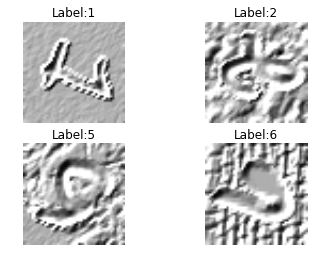
\includegraphics[scale=0.40]{sample_of_images.png}
	\caption{A sampling of the modified MNIST database}
	\label{MNISTSample}
\end{figure}

\section{Methodology}

We used the \href{http://www.numpy.org/}{NumPy package} and the \href{http://www.scikit-learn.org/}{scikit-learn library} to perform feature extraction and selection, implement our classifiers, and analyse our results. 

\subsection{Feature Extraction and Preprocessing}


\subsection{Feature Selection}

\subsection{Classification Algorithms}

\subsubsection{Baseline: Logistic Regression}
In Logistic Regression, we want to estimate the probability that some random vector $X=(x_1, \ldots, x_n)$ has a class $Y=y_k$, $P(Y=y_k | X=(x_1, \ldots, x_n))$. In the binary case we can derive the following using Bayes rule and conditioning:
\begin{equation*}
\begin{split}
&P(Y=1~|~X) = \frac{P(X, Y=1)}{P(X)}\\
&= \frac{ P(X~|~Y=1)\cdot P(Y=1) }{ P(X~|~Y=1)\cdot P(Y=1) + P(X~|~Y=0)\cdot P(Y=0) }\\
& = \frac{1}{1 + \exp{(-a)}} = \sigma(a) \text{~(Sigmoid Function)}\\
\end{split}
\end{equation*}

where $a=\ln\Big(\frac{P(Y=1~|~X)}{P(Y=0~|~X)}\Big)$ is the log-odds ratio. By approximating the log-odds ratio as a linear decision boundary of the features and weights, $w^T x$ we can use this as an estimate of the class being $Y=1$. We can optimize the Log-likelihood or Cross-Entropy function:

\begin{equation}
	\label{LL}
	L(w) = -\sum_{i=1}^n y_i\log\Big(\sigma(w^Tx_i)\Big) + (1-y_i)\log\Big(1-\sigma(w^Tx_i)\Big)
\end{equation}

and search for the optimal set of weights using the \emph{gradient descent algorithm} with $N$ steps and update rule \ref{LR_update_rule}:

\begin{equation}
\label{LR_update_rule}
	w_{k+1} = w_k + \alpha_k \sum_{i=1}^n \Big( x_i\big(y_i - \sigma(w_k^Tx_i\big) \Big)
\end{equation}


\subsubsection{Linear SVM}

\subsubsection{Fully Connected Feedforward Neural Network}

\subsubsection{Convolution Neural Network}
The convolution neural network \ref{LeCunn98} is a neural network with specialized layers in which not all neurons are connected to each other. Infact the main component is the subblayer (Fig \ref{convmaxlayer}) which contains the Convolution2D and MaxPool2d pair of layers. As shown in the (simplified) figure, the convolution conducted on the input is tranfromed into a 3D spatial arrangement of neurons. This is then subsampled (by selecting the MAX element from each subsection of the filter) to produce the set of outputs that can be reused in future layers.

Our experiments tested three variants of this using one, two and three Conv-Max sublayers coupled in the architechture shown in Fig \ref{CNNarch}

\begin{figure}[h]
	% \centering
	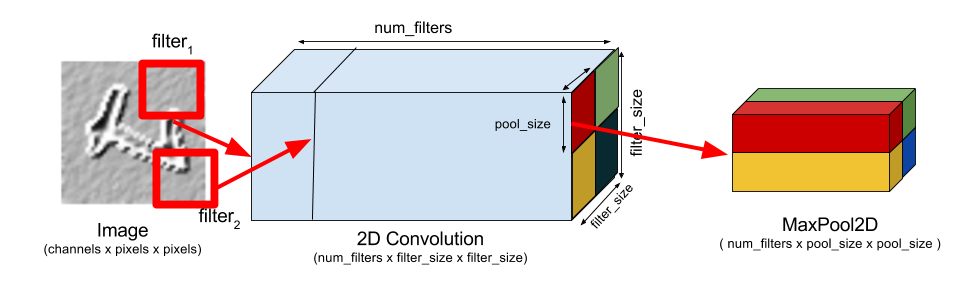
\includegraphics[scale=0.30]{convnet_example.png}
	\caption{A simplified example of the sublayer containing Convolution2D layer and a MaxPool2D layer. The variables correspond to the authors implementation of the network. The final network used one,two and three of these sublayers in tandem.}
	\label{convmaxlayer}
\end{figure}


\begin{figure}[h]
	\centering
	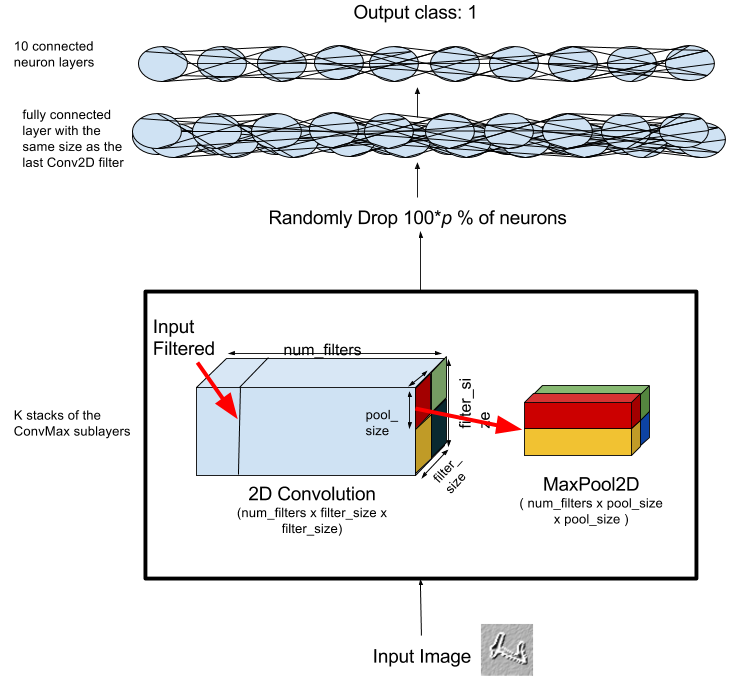
\includegraphics[scale=0.40]{architecture.png}
	\caption{The Convolution Neural Architechture included $k$ stacked sublayers shown in Fig \ref{convmaxlayer} connected to a dropout layer and finally fed into a fully connected layer containing $10$ neurons that did the final classification.}
	\label{CNNarch}
\end{figure}

\subsubsection{Spatial Transformer Network}

\subsection{Cross-Validation and Choice of Hyperparameters}

\section{Results}




\section{Discussion}

\subsection{Feature Extraction and Selection}



\subsection{Classifier Performance}

\subsection{Future Work}



\section{Statement of Contributions}

\section{Integrity of work}
We hereby state that all the work presented in this report is that of the authors.
\begin{thebibliography}{9}

\bibitem{LeCunn98}
Lecun Y., Bengio Y., and Haffner P.
 \emph{Gradient-Based Learning Applied to Document Recognition}
 Proceedings of the IEEE,
 1998.
\bibitem{ML_textcat}
 Sebastini, F.
  \emph{Machine Learning in Automated Text Categorization}
  ACM Computing Surveys (CSUR) 34
  2002.

\bibitem{CNN_committees}
 Claudiu D. and Meier U. et al.
  \emph{Convolutional Neural Network Committees For Handwritten Character
Classification}
  ACM Computing Surveys (CSUR) 34
  2002.

\bibitem{STN}
 Jaderberg, M., et al.
  \emph{Spatial Transformer Networks}
  ArXiv
  2015

\bibitem{MnistHome}
LeCun Y., Cortes, C. and Burges C.J.C.
	\emph{The MNIST Database of handwritten digits}
	http://yann.lecun.com/exdb/mnist/
% inspiration for graphic http://cs231n.github.io/convolutional-networks/
\end{thebibliography}

\end{document}
